%!TEX root = ../../thesis.tex

\section{Detecting atmospheres}
To help characterize an exoplanet, a detection of its atmosphere can provide useful information. After the detection of exoplanets and the measurement of bulk properties, detecting their atmospheres is the next step. The detection of planetary atmosphere is difficult due to the low planet-to-star flux ratio. This requires high precision instrumentation to detect. For example the planet-to-star flux ratio in the optical is $\approx 10^{-4}$ for a hot Jupiter with a 3 day orbit, in which the main component is reflected star light. In the infrared the thermal emission of the planets dominate and the flux ratio rises to $\approx 10^{-3}$. These flux ratios requires observations with signal-to-noise ratios of $10^4$ and $10^3$ in the optical and infrared respectively to achieve a planetary signal at the same level as the noise level. Only just at the capabilities of the current generation of technology, and with very long observation cost.


Several photometric and high-resolution spectroscopic techniques are showing promising results; detailed in the following sections.


\subsection{Occultation and phase variations}
Secondary transit and phase variations are an extension of the transit method, requiring higher precision to detect the reflection and thermal emission of the exoplanet. The observed light curve is analysed considering is has two components, not only light from the star but also light from the planet, albeit at a much lower flux level.
To help visualize and discuss the components of exoplanet atmospheres \fref{fig:transits_and_occultations} is provided showing a transiting planet in orbit around a star, in which the planet also passes behind the star causing an occultation. The planet is shown at several positions of the orbit indicating the proportion of dayside and night side observed.  Below the star and planet is a diagram showing the changing flux variation (solid black line) over time, following the orbit.  If the orbital alignment is such that the planet will pass behind the star it will cause an occultation of the planet. At this point the only light received is from the star alone, creating a baseline stellar measurement. While during the primary transit there is also a small thermal emission contribution from the night side of the planet, as well as it partially blocking the star.

\begin{figure}
    \centering
    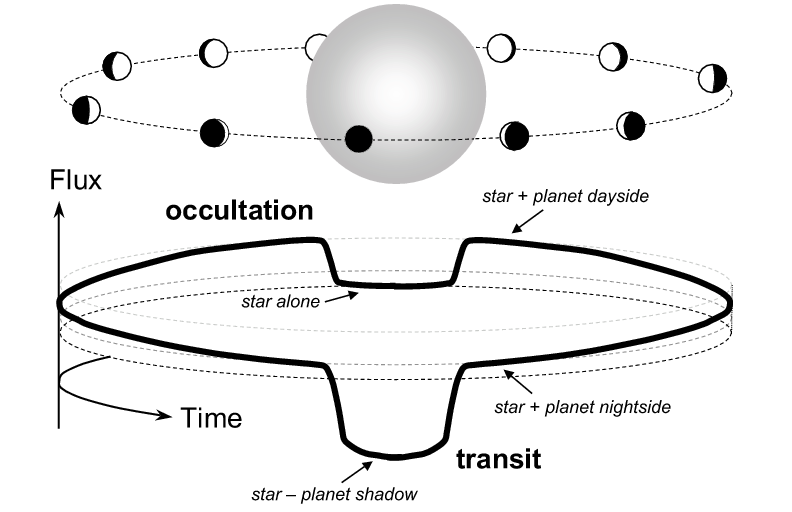
\includegraphics[width=0.6\linewidth]{./figures/introduction/circular_diagram.png}
    \caption{Illustration of the flux contribution from a star and planet in a transiting exoplanet system throughout its orbit. Credit~\citet{winn_transits_2010}}
    \label{fig:transits_and_occultations}
\end{figure}

Throughout the orbit of the planet there is a variation in the planetary flux due to the alternating day/night side of the planet observed. .
There are multiple components of the planetary flux, reflection and emission,  that can be analysed with multi-band phase curves \citep[e.g.][]{knutson_characterizing_2009, esteves_optical_2013}. Optical phase curves will mostly show the reflected light from the day side of the planet, allowing modelling the atmospheric albedo (fraction of light reflected by the atmosphere), and can provide details on the atmospheric scattering~\citep{madhusudhan_analytic_2012} and aerosol composition~\citep{oreshenko_optical_2016} through the optical phase function (day/night fraction). Thermal emission of the planet will provide stronger modulation of infrared phase curves and can provide insights into the atmospheres thermal
structure and heat circulation~\citep{ goodman_thermodynamics_2009, koll_temperature_2016}.


An example of phase variations in the infrared spectra of {WASP-43b} obtained with the Hubble Space telescope is given in \fref{fig:stevensonphasecurve2014}. The large amplitude of phase variation between the day and night side indicates that the night side is much cooler and there is an inefficient heat circularity from the day to night side. A planet with an efficient day/night heat distribution mechanism would quickly equalize and have smaller phase variation. One key observable from \fref{stevensonphasecurve2014} is that the peak of the phase variation is offset from the location of the secondary transit. The hottest part of the atmosphere does not correspond to the sub-stellar point i.e., the point of the planets surface closest to the star. Simulations of atmospheric circulation models find that this offset is caused by super-rotating equatorial jets which move the location of hottest point of the planet~\citep[e.g.][and references therein]{heng_atmospheric_2015}. 

\begin{figure}
    \centering
    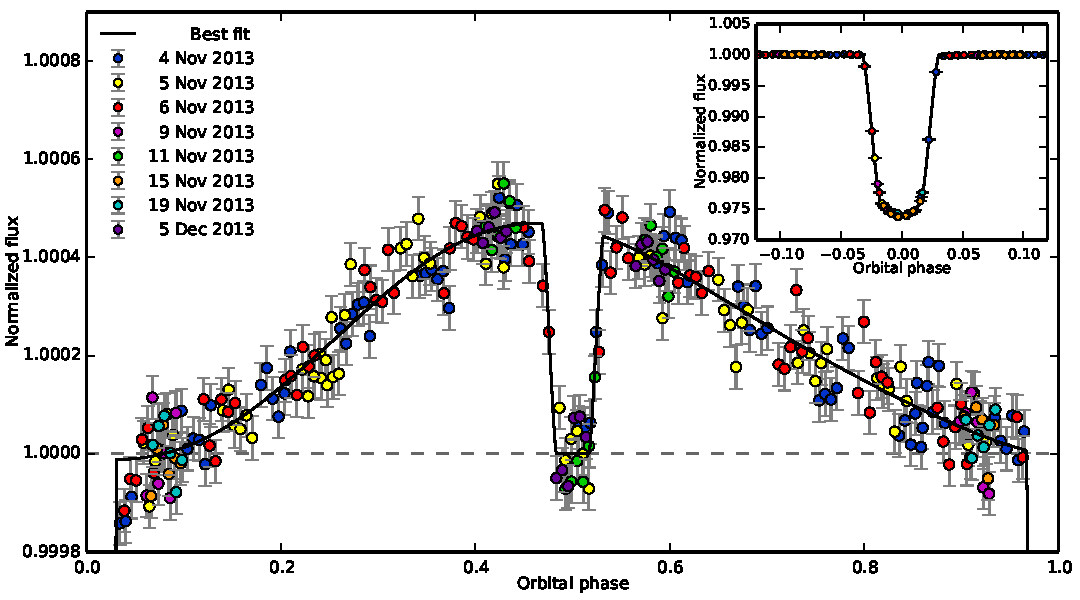
\includegraphics[width=0.6\linewidth]{figures/introduction/stevenson_phasecurve2014}
    \caption{Band integrated phase variation of WASP-43b from the HST - \cite{stevenson_thermal_2014}. The primary transit is inset top right.
        The peak of brightness occurs before the secondary transit, indicating heat distribution of the }
    \label{fig:stevensonphasecurve2014}
\end{figure}

The point of occultation, at which the planet is completely blocked by the star enables a baseline measurements for the star to be obtained without the planet. The depth of the occultation, is a direct measurement of the planet-to-star ratio between the star and the planet a \textbf{{cite secondary eclipse of reflectance, and secondary spectroscopy examples}.} Spectra obtained during the occultation will have no planetary signal and can be used remove the stellar component from spectra obtained at other phases to obtain the planetary spectrum.


The depth of the occultation is a measure of the flux from the day side of the planet which can indicate the atmospheric reflection and thermal emission of the planets atmosphere.


\todo{get a  thermal profile image/phase of hot spot?.}



\subsection{Transmission spectroscopy}
When a transiting planet crosses in-front of the host star it blocks out light from the star. However, when an atmosphere is present part of the light passes through  a planet with an atmosphere is not completely solid and parts
radius changes with wavelength, extra absorption during transit can give molecular composition.


transmission diagram? Snellen HORse talk?

Detection of winds



\citep{hoeijmakers_atomic_2018} detected Iron and titanium in ultra-hot Jupiter with Teff 4000K during transit.high resolution spectroscopy


The atmosphere is transparent to different wavelength at different heights in the atmosphere. Therefore the planetary radius is slightly different in different wavelength bands. This has shown ....



\subsection{High resolution spectroscopy}
Some key results from high res spectroscopy

Snellen  Brogi, de Kok

CRIRES  

Cross correlation mle  \citet{piskorz_evidence_2016}


For non-transiting planets ...  piskorz   with combiend stellar spectrum and planetary models.

